% Creating a simple Title Page in Beamer
\documentclass[aspectratio=169, 10pt]{beamer}
\usepackage{pgfpages}
\usepackage{booktabs}
% \usepackage{enumitem}
\usepackage{listings}
\usepackage{xcolor}
\usepackage[most]{tcolorbox}

% \setbeameroption{show notes on second screen=right}
% \setbeameroption{show only notes}
% Pacotes
\usepackage{lipsum}
\usepackage{graphicx}
\usepackage{color}
\usepackage[table]{xcolor}
\usepackage{tikz}
\usepackage{tcolorbox}
\usepackage{amsmath}
\usepackage{amsfonts}
\usepackage{amssymb}
\usepackage{mathrsfs}
\usepackage{mathtools}
\usepackage{enumitem} 
\usepackage{float}
% \usepackage[utf8]{inputenc}	
% \usepackage[vỉetnamese]{babel}
% \usepackage[utf8]{vietnam}
\usepackage{caption}
\usepackage{multirow}


% Theme choice:
\usetheme{CambridgeUS}

% Cores personalizadas
\definecolor{PROFMATgreen}{RGB}{0, 138, 163}
\definecolor{UFTgreen}{RGB}{0, 137, 124}
\definecolor{UFTblue}{RGB}{0, 84, 132}
\definecolor{UFTyellow}{RGB}{253, 185, 46}
\definecolor{UFTgray}{RGB}{132, 134, 136}

% Ativar numeração de tabelas
\setbeamertemplate{caption}[numbered]

% Definir novo estilo de item com quadrado verde
\setlist[itemize,1]{label=\textcolor{UFTgreen}{\rule{1ex}{1ex}}}

\setbeamercolor*{structure}{bg=UFTgreen,fg=black}

\setbeamercolor*{palette primary}{fg=black,bg=PROFMATgreen}
\setbeamercolor*{palette secondary}{fg=white,bg=UFTblue}
\setbeamercolor*{palette tertiary}{fg=black,bg=UFTgreen}
\setbeamercolor*{palette quaternary}{fg=white,bg=black}

\setbeamercolor{section in toc}{fg=black,bg=white}
\setbeamercolor{alerted text}{fg=white}

\setbeamercolor*{item}{fg=PROFMATgreen}

\setbeamercolor{block title}{bg=UFTgreen,fg=white}
\setbeamercolor{block body}{bg=UFTgray!10,fg=black}

\setbeamercolor{titlelike}{fg=white, bg=UFTblue}
\setbeamercolor{frametitle}{bg=UFTgray!20,fg=UFTgreen}



\setbeamertemplate{background}{
    \parbox[c][\paperheight][c]{\paperwidth}{
        \vfill
        \includegraphics[width=\paperwidth,height=\paperheight,keepaspectratio]{img/general/background.png} 
        \vfill
    }
}


% Customizar a página de título
\setbeamertemplate{title page}{
\vbox{}
\begin{center}
    \begin{minipage}{0.3\linewidth}
        \centering
    \end{minipage}
\end{center}
    
    %\vfill
    % \vskip1em\par
    \begingroup
        \centering
        \begin{beamercolorbox}[sep=8pt,center,shadow=true,rounded=false]{title}
            \usebeamerfont{title}\inserttitle\par%
            \ifx\insertsubtitle\@empty%
            \else%
                \vskip0.25em%
                {\usebeamerfont{subtitle}\usebeamercolor[fg]{subtitle}\insertsubtitle\par}%
            \fi%
        \end{beamercolorbox}%
        \vskip0.5em\par
        \begin{beamercolorbox}[sep=6pt,center]{author}
            \usebeamerfont{author}\insertauthor
        \end{beamercolorbox}
        % \vskip0.1em\par
        % \begin{beamercolorbox}[sep=5pt,center]{email}
        %     \usebeamerfont{institute} \insertemail
        % \end{beamercolorbox}
        % \vskip0.2em\par
        % \begin{beamercolorbox}[sep=5pt,center]{advisor}
        %     \usebeamerfont{institute} \advisorname
        % \end{beamercolorbox}
        \vskip0.2em\par
        \begin{beamercolorbox}[sep=5pt,center]{institute}
            \usebeamerfont{institute}\insertinstitute
        \end{beamercolorbox}
        \vskip0.2em\par
        \begin{beamercolorbox}[sep=5pt,center]{date}
            \usebeamerfont{institute}\insertdate
        \end{beamercolorbox}
        \vskip0.5em\par
    \endgroup
    \vfill
}


% % Ẩn biểu tượng điều hướng
\setbeamertemplate{navigation symbols}{}

% Màu & cỡ chữ cho footer
\setbeamercolor{author in head/foot}{bg=UFTgreen, fg=black}
\setbeamercolor{title  in head/foot}{bg=UFTblue,  fg=white}
\setbeamercolor{date   in head/foot}{bg=UFTgreen, fg=black}
\setbeamerfont{author in head/foot}{size=\footnotesize}
\setbeamerfont{title  in head/foot}{size=\footnotesize}
\setbeamerfont{date   in head/foot}{size=\footnotesize}


% Footline tuỳ biến (3 cột)
\setbeamertemplate{footline}{%
  \leavevmode
  \hbox{%
    % Cột trái: tác giả ngắn
    \begin{beamercolorbox}[wd=.33\paperwidth,ht=2.5ex,dp=1.1ex,center]{author in head/foot}%
      \hspace*{1ex}\insertshortauthor
    \end{beamercolorbox}%
    % Cột giữa: short title, tự xuống dòng khi dài
    \begin{beamercolorbox}[wd=.47\paperwidth,ht=2.5ex,dp=1.1ex,center]{title in head/foot}%
      \parbox{\dimexpr.45\paperwidth\relax}{\centering\insertshorttitle}%
    \end{beamercolorbox}%
    % Cột phải: ngày + số trang
    \begin{beamercolorbox}[wd=.20\paperwidth,ht=2.5ex,dp=1.1ex,center]{date in head/foot}%
      \hspace{4ex} \insertshortdate\hspace{10ex}\insertframenumber{} / \inserttotalframenumber\hspace{1ex}%
    \end{beamercolorbox}%
  }%
  \vskip0pt%
}



% Remover bordas arredondadas dos blocks
\makeatletter
\setbeamertemplate{blocks}[default] % Isso remove o arredondamento
\makeatother


% Pacotes de citações
% ---

\usepackage[alf,abnt-etal-text=it,abnt-repeated-author-omit=yes,abnt-etal-list=0,abnt-etal-cite=3,abnt-emphasize=bf]{abntex2cite}	% Citações padrão ABNT



\setbeamercolor{bibliography entry author}{fg=black}
\setbeamertemplate{bibliography item}{\newblock}


\setbeamertemplate{frametitle continuation}{}

% Redefinir o separador para um traço
% Redefinir o separador
\captionsetup[figure]{labelformat=simple, labelsep=endash, textformat=period, font=footnotesize}
\captionsetup[table]{labelformat=simple, labelsep=endash, textformat=period, font=footnotesize}


% Redefine espaçamento antes e depois da legenda em figuras e tabelas
\captionsetup[figure]{aboveskip=2pt, belowskip=0pt}
\captionsetup[table]{aboveskip=2pt, belowskip=0pt}


% Define uma penalidade alta para a hifenização
\hyphenpenalty=10000
\tolerance=10000


% Personalizando o estilo da tabela de conteúdos
\setbeamertemplate{section in toc}[sections numbered]
\renewcommand{\thesection}{\textcolor{PROFMATgreen}{\arabic{section}}}
\renewcommand{\thesubsection}{\textcolor{PROFMATgreen}{\arabic{section}.\arabic{subsection}}}

\setbeamersize{text margin left=0.8cm, text margin right=0.8cm}


\usepackage{tcolorbox}

\newtcbox{\code}{on line, 
    arc=2pt,                % Độ bo tròn góc
    colback=gray!20,        % Màu nền (xám nhạt)
    colframe=gray!20,       % Viền cùng màu nền
    boxrule=0pt,            % Không độ dày viền
    boxsep=0pt, left=2pt, right=2pt, top=2pt, bottom=2pt, % Khoảng cách đệm
    fontupper=\ttfamily     % Font chữ kiểu code
}

\newtcolorbox{softbox}{
    colback=black!3,        % Màu nền: Xám rất nhạt (3% đen)
    colframe=black!3,       % Màu viền: Trùng màu nền (để không thấy viền)
    arc=8pt,                % Độ bo tròn góc
    boxrule=0pt,            % Độ dày viền = 0
    left=10pt, right=10pt, top=8pt, bottom=8pt, % Khoảng cách lề bên trong
    fontupper=\itshape\color{black!80} % Font chữ: Nghiêng và màu xám đậm (80% đen)
}

\definecolor{codegreen}{rgb}{0,0.6,0}
\definecolor{codegray}{rgb}{0.5,0.5,0.5}
\definecolor{codepurple}{rgb}{0.58,0,0.82}
\definecolor{backcolour}{rgb}{0.95,0.95,0.92}

\definecolor{termBG}{HTML}{0C1C23}    % Màu nền xanh đen đậm
\definecolor{termRed}{HTML}{FF5555}   % Màu đỏ
\definecolor{termYellow}{HTML}{F1FA8C}% Màu vàng
\definecolor{termWhite}{HTML}{F8F8F2} % Màu chữ trắng sáng
\definecolor{termGray}{HTML}{A9B7C6}  % Màu xám nhạt (nếu cần)

\newtcolorbox{TerminalBox}{
    colback=termBG,       
    coltext=termWhite,    
    boxrule=0pt,          
    arc=3pt,              
    left=4pt, right=4pt, top=4pt, bottom=4pt, % Giảm lề đệm xuống 4pt cho gọn
    % QUAN TRỌNG: Dùng \tiny để chữ siêu nhỏ
    fontupper=\ttfamily\scriptsize\linespread{1.0}\selectfont, 
    enhanced
}

% Lệnh tắt để tô màu cho nhanh
\newcommand{\cred}[1]{\textcolor{termRed}{#1}}
\newcommand{\cyellow}[1]{\textcolor{termYellow}{#1}}

% Cấu hình style cho C++
\lstdefinestyle{mystyle}{
    backgroundcolor=\color{backcolour},   
    commentstyle=\color{codegreen},
    keywordstyle=\color{magenta},
    numberstyle=\tiny\color{codegray},
    stringstyle=\color{codepurple},
    basicstyle=\ttfamily\footnotesize, % Font chữ kiểu máy đánh chữ, kích thước nhỏ
    breakatwhitespace=false,         
    breaklines=true,                 % Tự động xuống dòng nếu quá dài
    captionpos=b,                    
    keepspaces=true,                 
    numbers=left,                    % Hiển thị số dòng bên trái
    numbersep=5pt,                  
    showspaces=false,                
    showstringspaces=false,
    showtabs=false,                  
    tabsize=2,                       % Độ rộng tab = 2 spaces
    language=C++                     % Ngôn ngữ C++
}

\lstset{style=mystyle}

% Informações do documento
\title[Object-Oriented Programming - Design Pattern]{\large \textbf{Prototype Design Pattern - A Way to Clone an Object}}
% \subtitle{}
\author[Khang P., Nghia T., Cao C. and Nhat H.]{Khang P. Nguyen \inst{1}, Nghia T. Hoang \inst{1}, Cao C. Phan \inst{1} and Hoang N. Nguyen \inst{1}}
\institute[]{
\inst{1}University of Science - Vietnam National University\\
}
% Definir o nome do orientador
% \newcommand{\advisorname}{}
\begin{document}
\begin{frame}
    \titlepage
\end{frame}

\begin{frame}[t]
    \frametitle{Outline}
    \tableofcontents
    \note{
    \begin{itemize}
        \item Here is the outline of my presentation.
        \item I will begin with an introduction to the problem and its motivation, followed by a review of related works.
        \item Then, I will present our proposed methodology, experimental setup, and results.
        \item Finally, I will conclude with the main findings and possible directions for future research.
    \end{itemize}
    }
\end{frame}

\section{Introduction}
Trong lĩnh vực thiết kế phần mềm riêng và lập trình hướng đôi tượng nói chung thì việc áp dụng design pattern vào dự án thực tế là rất cần thiết, vì nó cho phép ta có thể tái sử dụng và có các giải pháp được chứng minh đối với các bài toán thường gặp trong quá trình thiết kế và triển khai các hệ thống phần mềm. 
Design pattern là các giải pháp tổng quát đối với các vấn đề thường gặp xuất phát trong quá tình kiểm thử và phát triển hệ thống phần mềm. Nó cung cấp một tập các giải pháp đã được chứng minh cho các thử thách trong thiết kế và tối ưu các phương pháp tốt nhất cho việc phát triển phần mềm.

Design pattern được chia thành 3 nhóm khác nhau: \textbf{Creational, Structural, Behavioral}. Mỗi loại đều có những vai trò và nhiệm vụ khác nhau chẳng hạn như \textbf{Creational} sẽ trừu tượng hóa các quá trình khởi tạo, \textbf{Structural} sẽ liên quan tới các class và objects được kết hợp như thế nào để tạo thành các cấu trúc lớn hơn, hay đối với \textbf{Behavioral} thì sẽ liên quan tới các thuật toán và phân công trách nhiệm giữa các đối tượng.
Và trong các loại trên, bài báo cáo này sẽ tập trung vào \textbf{Prototype} thuộc loại \textbf{Creational}. Đây là một trong những pattern phổ biến và mạnh mẽ ở trong các quy trình phát triển phần mềm. Nó cung một giải pháp tiện lợi, nhanh chóng và hiệu quả để có thể khởi tạo một object phức tạp, có thể bỏ qua được loại của lớp, cũng như là không cần biết quá chi tiết về logic bên trong của class đó \cite{gfg_prototype}.

\section{GitHub Repository Link}
Nhằm phục vụ cho việc quản lý dự án, cũng như là công khai các mã nguồn có trong dự án thì nhóm cũng đã đẩy toàn bộ dự án lên trên \href{https://github.com/}{GitHub}:

\textbf{Link: } \href{https://github.com/khang1108/prototype-design-pattern}{See more}

\section{GitHub Commit List}
Để cung cấp một cái nhìn minh bạch và toàn diện về quá trình phát triển của dự án, dưới đây là toàn bộ lịch sử commit được trích xuất từ repository. Danh sách này được trình bày theo định dạng rút gọn, thể hiện các thay đổi, gộp nhánh và các cột mốc quan trọng từ khi bắt đầu cho đến khi hoàn thiện dự án.

% Sử dụng môi trường figure để có caption và label, giúp nó không bị tách rời
\begin{figure}[htbp]
% Sử dụng lstlisting để hiển thị code một cách ổn định và an toàn
\begin{lstlisting}[
    language=bash, 
    basicstyle=\ttfamily\scriptsize, % Font chữ TINY (rất nhỏ) để chứa được toàn bộ log
    breaklines=true,         % Tự động xuống dòng khi cần
    frame=single,            % Thêm khung bao quanh
    caption={Lịch sử commit đầy đủ của dự án NaTruKi},
    label=lst:gitlog_full
]
commit a6e0fa047fe45823b7a9c6bdf619f8a54add5b44 (HEAD -> main, origin/main)
Merge: 46ccd09 70bc072
Author: Nguyen Phuc Khang <nguyenphuc.khang110806@gmail.com>
Date:   Mon Dec 1 23:50:45 2025 +0700

    Merge branch 'main' of https://github.com/khang1108/prototype-design-pattern

commit 46ccd097e39a24cde396dc24b6ff031c96ea81dc
Author: Nguyen Phuc Khang <nguyenphuc.khang110806@gmail.com>
Date:   Mon Dec 1 23:46:17 2025 +0700

    Initial commit

commit 70bc072e9e8158615007d6e5bb19ef252ece207b
Author: Nguyen Phuc Khang <94360818+khang1108@users.noreply.github.com>
Date:   Mon Dec 1 23:42:18 2025 +0700

    Initial commit

\end{lstlisting}
\end{figure}

\section{GitHub Contribution}
Bằng việc sử dụng GitHub để quản lý dự án, cũng như là tổ chức và xây dựng thì nhóm cũng đã có thể ghi lại những hoạt động và đóng góp của từng thành viên như sau:

\begin{figure}[h!]
  \centering
  \includegraphics[width=0.8\textwidth]{images/github_stats.jpg}
  \caption{GitHub Contributions stats}
  \label{fig:github_stats}
\end{figure}

Qua hình ảnh này, ta có thể thấy được mức độ hoạt động của các thành viên trong nhóm. Vì dự án này không quá nặng về code nên mà thiên về tìm hiểu nội dung, các thành viên chủ yếu hoạt động bên \href{docs.google.com}{Google Docs} nên trên Github sẽ không quá nổi bật.

% --- THÊM LỆNH NÀY VÀO ---
\FloatBarrier 
% -------------------------

\section{Class Diagram}
Để trực quan hóa được ý tưởng về các tổ chức và xây dựng dự án này của nhóm thì ta có thể xem qua \textit{Class Diagram} - \textit{Unified Model Language (UML)}, đây chính là sơ đồ tổng thể toàn bộ các mối quan hệ của các class có trong dự án, cũng như là các thuộc tính, các phương thức được xây dựng cho mỗi class.

\begin{figure}[H]
  \centering
  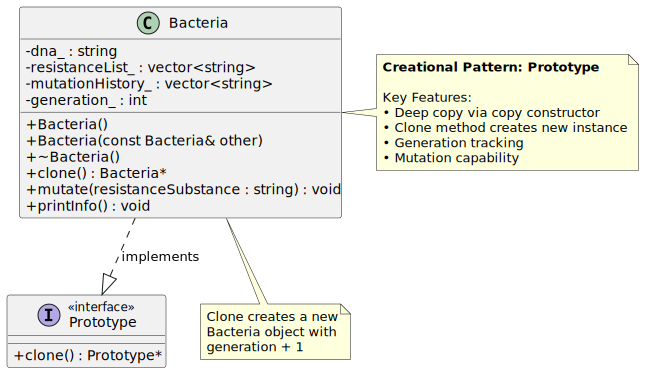
\includegraphics[width=\textwidth]{images/bacteria_plantuml.png}
  \caption{Bacteria UML Class Diagram}
  \label{fig:bacteria_uml}
\end{figure}

% --- THÊM LỆNH NÀY VÀO ---
\FloatBarrier 
% -------------------------

\begin{figure}[H]
    \centering
    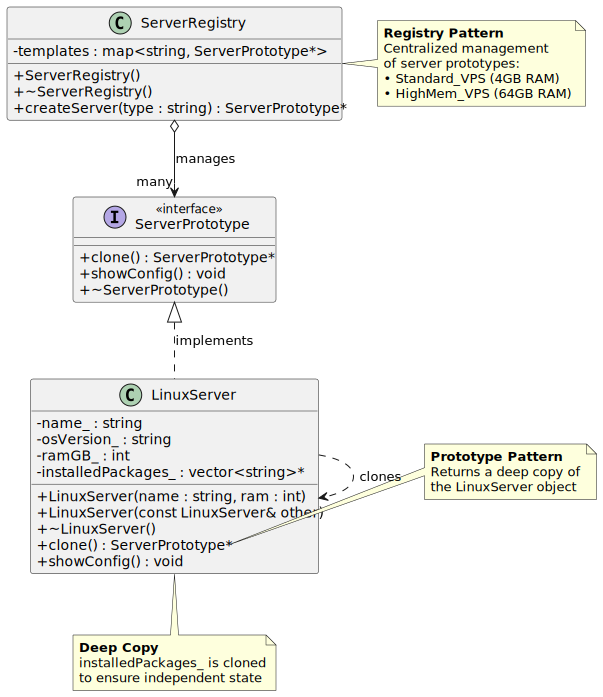
\includegraphics[width=\textwidth]{images/registry_plantuml.png}
    \caption{Registry Prototype UML Class Diagram}
    \label{fig:registry_uml}
\end{figure}

% --- THÊM LỆNH NÀY VÀO ---
\FloatBarrier 
% -------------------------

\subsection{Basic Prototype Implementation}
\subsubsection{Định nghĩa}
Đây là dạng thuần túy của mẫu thiết kế Prototype, nó tập trung vào kỹ thuật \textbf{Tự nhân bản}. Cấu trúc của nó bao gồm 3 phần chính đó là \textbf{Client}, \textbf{Prototype Interface} và \textbf{Concrete Prototype} với các nhiệm vụ khác nhau như sau \cite{patterns_prototype}:

\FloatBarrier 

\begin{figure}
  \includegraphics[width=\textwidth]{images/basic_implementation.jpg}
  \caption{Cấu trúc của Basic Prototype Implementation}
  \label{label:structure_basic_prototype}
\end{figure}

\begin{itemize}
  \item \textbf{Prototype Interface:} Cấu trúc này có nhiệm vụ là định nghĩa các phương thức cho việc nhân bản \textit{cloning} các đối tượng và đặt các tiêu chuẩn sao cho tất cả các \textbf{concrete prototypes} phải tuân theo. Nó bao gồm một phương thức \code{clone()} là nơi mà các \textbf{concrete prototypes} sẽ triển khai để tạo một bản sao của nó.
  \item \textbf{Concrete Prototypes:} Lớp này sẽ triển khai các \code{prototype interface} hoặc là mở rộng lớp trừu tượng. Nó biểu diễn một đối tượng có kiểu đặc biệt có thể được nhân bản.
  \item \textbf{Client:} Người dùng là đoạn mã nguồn hoặc là một module nào đó sẽ yêu cầu việc khởi tạo một đối tượng bới bằng cách giao tiếp với \textbf{prototype}.
  \item \textbf{Clone method:} Đây sẽ là phương thức được định nghĩa bên trong \code{prototype interface} hoặc là \code{abstract class} và chỉ ra rằng một đối tượng phải được nhân bản như nào. Các \code{concrete prototypes} sẽ triển khai phương thức này để định nghĩa thuộc tính nhân bản riêng biệt cho bản thân nó.
\end{itemize}

\FloatBarrier
\begin{figure}[H]
  \centering
  \includegraphics[width=0.9\textwidth]{images/analogy_example.jpg}
  \caption{Hình ảnh ẩn dụ cho Prototype}
  \label{label:anology_img}
\end{figure}

\FloatBarrier
Chẳng hạn như hình ảnh ẩn dụ thực tế về Protype ở trên, ban đầu ta có một mẫu được gọi là \code{Prototype} có các thuộc tính và thông tin cơ bản về class này. Sau đó \code{Client} sẽ tiến hành gọi \code{clone()} để có thể nhân bản ra các bản sao khác để tạo ra thêm các mẫu rời rạc khác từ đó mà có thể tùy chỉnh các thông tin cho các mẫu đó.

Việc áp dụng Prototype không chỉ giúp cho \code{Client} có thể dễ dàng khởi tạo một đối tượng mới dựa trên đối tượng mẫu mà không cần biết chi tiết về bên trong lớp đó có những gì. Từ đó mà giúp cho code của ta có thể gọn hơn, dễ chỉnh sửa cũng như là sửa lỗi. Tóm gọn lại Protype sẽ có các lợi ích như sau \cite{faraz_prototype_proscons}:
\begin{itemize}
  \item \textbf{Efficient Object Creation:} Prototype pattern cho phép ta một cách khởi tạo các object một cách hiểu quả hơn thông qua việc cho phép các đối tượng có thể \code{clone()} thay vì là khởi tạo từ đầu. Nó có thể cải thiện hiệu suất một cách mạnh mẽ, đặc biệt là nếu các đối tượng phức tạp.
  \item \textbf{Reduced Subclassing:} Thay vì là ta phải tạo nhiều subclass khác nhau để tạo các đối tượng khác nhau, thì với \code{Prototype} thì ta chỉ cần xây dựng phương thức \code{clone()}. Nó giúp ta giải được sự bùng nổ subclass, cũng như là đơn giản hóa các lớp kế thừa và làm cho \code{codebase} có thể dễ bảo trì hơn.
  \item \textbf{Flexibility:} Nhân bản các đối tượng cho phép ta có thể tùy chỉnh các thông tin đối tượng một cách độc lập, cũng như là thay đổi \code{dynamic runtime changes} không ảnh hưởng tới đối tượng nguyên bản. 
  \item \textbf{Promotes Reusability:} Bằng cách cung cấp các kỹ thuật \code{clone} thì \code{Prototype} pattern có thể tái sử dụng. Các đối tượng được nhân bản có thể bảo toàn như là các mẫu ban đầu với sự tương đồng về thuộc tính, hành vi, từ đó mà có thể tiết kiệm thời gian và nguồn lực.
\end{itemize}

\subsubsection{Code Demo}
\begin{lstlisting}
  #include <iostream>
  #include <vector>
  #include <string>

  #define RED "\033[31m"
  #define YELLOW "\033[33m"
  #define GREEN "\033[32m"
  #define RESET "\033[0m"

  class Bacteria{
  private:
      std::string dna_;
      std::vector<std::string> resistanceList_;
      std::vector<std::string> mutationHistory_;
      int generation_;
  public:
      /// @brief : Default constructor
      Bacteria() : dna_(""), resistanceList_({}), mutationHistory_({}), generation_(0){
          std::cout << "\n[INFO] Initialize a " << RED << "'bacteria'" << RESET << " object via " << 
                  YELLOW << "'default constructor'" << RESET << '\n';
      } 
      /// @brief : Copy constructor using Deep Copy
      Bacteria(const Bacteria& other){
          dna_ = other.dna_;
          resistanceList_ = other.resistanceList_;
          mutationHistory_ = other.mutationHistory_;
          generation_ = other.generation_;

          std::cout << "\n[INFO] Initialize a " << RED << "'bacteria'" << RESET << " object via " << 
                  YELLOW << "'copy constructor'" << RESET << '\n';
      }
      /// @brief : Destructor
      ~Bacteria(){
          std::cout << "\n[INFO] Deleting the" << RED << "'bacteria'" << RESET << " object\n";
      }
      /// @brief : Clone method
      Bacteria* clone() {
          std::cout << "Cloning " << RED << "'bacteria'" << RESET << " object via " 
                  << YELLOW << "'clone()'" << RESET << "method\n"; 

          Bacteria* newBacteria = new Bacteria(*this);

          newBacteria->generation_ = this->generation_ + 1;

          return newBacteria;
      }

      ///< @brief : Mutating 
      void mutate(const std::string& resistanceSubstance) {
          this->dna_ += "_Mutated";
          this->resistanceList_.push_back("Resist-" + resistanceSubstance);
          this->mutationHistory_.push_back("Mutate-" + resistanceSubstance);
      }

      void printInfo() {
          std::cout << "--- Bacteria Info ---" << "\n";
          std::cout << "Gen: " << dna_ << "\n";
          std::cout << "Generation: " << generation_ << "\n";
          std::cout << "Resistance: ";
          for (const auto& r : resistanceList_) std::cout << r << " ";
          std::cout << "\n" << "\n";
      }
  };
  int main()
  {
      std::ios_base::sync_with_stdio(false);

      Bacteria* mother = new Bacteria();

      mother->mutate("Penicillin");      
      mother->mutate("Ampicillin");     
      mother->mutate("Tetracycline");    
      mother->mutate("Streptomycin");    

      std::cout << "Mother after mutated:" << std::endl;
      mother->printInfo();

      std::cout << "Child cloned from Mother:" << std::endl;
      Bacteria* child = mother->clone();

      child->mutate("Chloramphenicol");

      child->printInfo();

      delete child;
      delete mother;

      return 0;
  }
\end{lstlisting}

\subsubsection{Output}
\begin{TerminalBox}
% --- DÒNG 1: KHỞI TẠO MẸ ---
[INFO] Initialize a \cred{'bacteria'} object via \cyellow{'default constructor'} \\
Mother after mutated: \\
--- Bacteria Info --- \\
Gen: \_Mutated\_Mutated\_Mutated\_Mutated \\
Generation: 0 \\
Resistance: Resist-Penicillin Resist-Ampicillin Resist-Tetracycline Resist-Streptomycin \\[1em]

% --- DÒNG 2: CLONE ---
Child cloned from Mother: \\
Cloning \cred{'bacteria'} object via \cyellow{'clone()'} method \\[1em]

% --- DÒNG 3: KẾT QUẢ CON ---
[INFO] Initialize a \cred{'bacteria'} object via \cyellow{'copy constructor'} \\
--- Bacteria Info --- \\
Gen: \_Mutated\_Mutated\_Mutated\_Mutated\_Mutated \\
Generation: 1 \\
Resistance: Resist-Penicillin Resist-Ampicillin Resist-Tetracycline Resist-Streptomycin Resist-Chloramphenicol
\end{TerminalBox}

\subsection{Registry Prototype Implementation}
Đây là dạng mở rộng hơn của Prototype, ta tiến hành kết hợp 2 pattern lại với nhau cụ thể trong trường hợp này là kết hợp giữa \code{Registry} và \code{Prototype} pattern. Mục tiêu của việc triển khai này sẽ tập trung vào việc ta có thể \textbf{quản lý và tái sử dụng}. Nó cung cấp cho ta một cách để có thể truy cập các \code{Prototype} thường dùng. Các \code{Prototypes} ấy sẽ được lưu trữ trong một tập hợp được xây dựng từ trước và luôn sẵn sàng để có thể được nhân bản \cite{ramjas_prototype}. 

\FloatBarrier

\begin{figure}
  \includegraphics[width=0.9\textwidth]{images/registry_implementation.jpg}
  \caption{Cấu trúc cho Registry Implementation}
  \label{label:registry}
\end{figure}

\FloatBarrier
Trong cấu trúc này ta sẽ tạo thêm một lớp \code{PrototypeRegistry} để có thể lưu trữ các 

\subsubsection{Registry Pattern}
Registry Pattern là một hướng đi \code{cấu trúc hóa} được sử dụng để tập trung hóa và quản lý truy cập tới các phần tử được chia sẻ hoặc là các phiên bản bên trong một phần mềm\cite{gfg_registry}. Mẫu thiết kế này nó liên quan tới việc khởi tạo một \code{registry} (thanh ghi) là kho lưu trữ trung tâm hoặc toàn cục, nơi các đối tượng sẽ đăng ký và lưu trữ với các mã định danh duy nhất.

Việc kết hợp \code{Registry} và \code{Prototype} tạo cho ta sự tiện lợi khi nó đã tiền xây dựng sẵn và khi cần ta chỉ cần truy cập tới đối tượng ta cần nhân bản thông quan một \code{key}, thông thường các đối tượng ấy sẽ được lưu trữ bên trong một \code{Hash Map}. Nhờ sự kết hợp đó nó cho ta thấy được các lợi ích như sau:
\begin{itemize}
  \item \textbf{Access Efficiency:} Khi được triển khai đúng cách, \code{Registry} sẽ cho ta thấy được hiệu quả được cải thiện rõ rệt bằng việc cung cấp một các truy cập tối ưu đến các tài nguyên được chia sẻ. Các thành phần sẽ có thể được truy vấn các đối tượng một cách nhanh chóng từ thanh ghi mà không cần phải khởi tạo hoặc là tra cứu chúng nhiều lần.
  \item \textbf{Caching and Optimizations:} \code{Registry} có thể kết hợp với các chiến lược lưu bộ nhớ đệm \code{caching} để tối ưu hiệu quả. Nhờ vào điều này mà nhu cầu về các truy vấn lặp đi lặp lại và khởi tạo các đối tượng được giảm đi rõ rệt.
  \item \textbf{Centralized Resource Management:} Nhờ vào việc tập trung các tài nguyên chia sẻ vào một chỗ tại \code{Registry}, nên mẫu thiết kế này có thể đơn giản hóa cho việc tinh chỉnh quá trình có thể thêm hoặc bớt một cách dễ dàng. Thay vì là ta phải quản lý các nguồn tài nguyên trên nhiều đối tượng, nhiều nodes khác nhau thì bây giờ tất cả đều tập trung tại một \code{Registry} đơn lẻ.
\end{itemize}

\subsubsection{Demo Code}
\begin{lstlisting}
  #include <iostream>
  #include <string>
  #include <map>
  #include <thread>
  #include <chrono>
  #include <map>
  #include <vector>

  #define RED "\033[31m"
  #define YELLOW "\033[33m"
  #define GREEN "\033[32m"
  #define RESET "\033[0m"

  class ServerPrototype
  {
  public:
      ///< @brief: Pure virtual allowing each subclass to define its own method
      virtual ServerPrototype* clone() const = 0;
      virtual void showConfig() = 0;
      virtual ~ServerPrototype() {}
  };

  class LinuxServer : public ServerPrototype {
  private:
      std::string name_;
      std::string osVersion_;
      int ramGB_;
      std::vector<std::string>* installedPackages_;
  public:
      LinuxServer(std::string name, int ram) : name_(name), ramGB_(ram) {
          this->osVersion_ = "Linux 6.17.4-arch2-1";
          installedPackages_ = new std::vector<std::string>{"nginx", "mysql", "php"};

          std::cout << "[System] Installing OS for Prototype " << name_ 
                  << "via " << RED << "'default  constructor'" << RESET << '\n';
      }

      LinuxServer(const LinuxServer& other){
          name_ = other.name_;
          osVersion_ = other.osVersion_;
          ramGB_  =  other.ramGB_;

          installedPackages_ =  new std::vector<std::string>(*other.installedPackages_);

          std::cout << "[System] Installing OS for Prototype " << name_ 
                  << "via " << RED << "'copy  constructor'" << RESET << '\n';
      }

      ServerPrototype* clone() const override {
          return new LinuxServer(*this);
      }

      void showConfig() override {
          std::cout << "Server: " << name_ << " | OS: " << osVersion_ << " | RAM: " << ramGB_ << "GB" << std::endl;
      }

      ~LinuxServer(){
          delete installedPackages_;
      }
  };

  class ServerRegistry
  {
  private:
      std::map<std::string,  ServerPrototype*> templates;

  public:
      ServerRegistry() {
          std::cout <<  "=== STARTING REIGSTRY ===" << std::endl;

          templates["Standard"] = new LinuxServer("Standard_VPS", 4);
          templates["HighMem"] = new LinuxServer("HighMem_VPS", 64);

          std::cout << "=== COMPLETED INITIALIZATION ===" << std::endl;
      }

      ~ServerRegistry() {
          for (auto const& [key, val] : templates) {
              delete val;
          }
          templates.clear();
      }

      ServerPrototype* createServer(std::string type){
          if(templates.find(type) != templates.end()){
              return templates[type]->clone();
          }
          return nullptr;
      }
  };

  int main() {
      std::ios_base::sync_with_stdio(false);

      ServerRegistry registry;

      std::cout << "[INFO] Create a " << RED << "'Standard'" << RESET 
              << " server\n";
      ServerPrototype* standardServer = registry.createServer("Standard");
      if(standardServer) standardServer->showConfig();

      std::cout << "[INFO] Create a " << RED << "'HigMem'" << RESET 
              << " server\n";
      ServerPrototype* highMem = registry.createServer("HighMem");
      if(highMem) highMem->showConfig();

      std::cout << "[INFO] Create a " << RED << "'Standard'" << RESET 
              << " server\n";
      ServerPrototype* standardServer2 = registry.createServer("Standard");
      if(standardServer2) standardServer2->showConfig();

      delete standardServer;
      delete highMem;
      delete standardServer2;

      return 0;
  }
\end{lstlisting}

\subsubsection{Output}
    \begin{TerminalBox}
    === STARTING REIGSTRY === \\
    ~[System] Installing OS for Prototype Standard\_VPSvia \cred{'default  constructor'} \\
    ~[System] Installing OS for Prototype HighMem\_VPSvia \cred{'default  constructor'} \\
    === COMPLETED INITIALIZATION === \\[0.5em]
    
    ~[INFO] Create a \cred{'Standard'} server \\
    ~[System] Installing OS for Prototype Standard\_VPSvia \cred{'copy  constructor'} \\
    Server: Standard\_VPS | OS: Linux 6.17.4-arch2-1 | RAM: 4GB \\[0.5em]
    
    ~[INFO] Create a \cred{'HigMem'} server \\
    ~[System] Installing OS for Prototype HighMem\_VPSvia \cred{'copy  constructor'} \\
    Server: HighMem\_VPS | OS: Linux 6.17.4-arch2-1 | RAM: 64GB \\[0.5em]
    
    ~[INFO] Create a \cred{'Standard'} server \\
    ~[System] Installing OS for Prototype Standard\_VPSvia \cred{'copy  constructor'} \\
    Server: Standard\_VPS | OS: Linux 6.17.4-arch2-1 | RAM: 4GB
    \end{TerminalBox}
\section{Feature Checklist}

\begin{table}[H]
    \centering
    \renewcommand{\arraystretch}{1.5}
    \caption{Checklist các hạng mục công việc cần thực hiện}
    \label{tab:checklist}
    \begin{tabular}{@{} l c p{7cm} c c @{}}
        \toprule
        \textbf{Danh mục} & \textbf{ID} & \textbf{Nội dung công việc} & \textbf{Ưu tiên} & \textbf{Trạng thái} \\
        \midrule
        
        Documentation & D.1 & \textbf{Main Report}: Viết báo cáo chính của dự án. & M & Done \\
                      & D.2 & \textbf{Slide}: Thiết kế slide thuyết trình. & M & Done \\
        
        \addlinespace[0.5em] 
        
        Implementation & C.1 & \textbf{Basic Prototype Demo Code}: Cài đặt mẫu Prototype cơ bản. & M & Done \\
                       & C.2 & \textbf{Registry Prototype Demo Code}: Cài đặt Registry quản lý mẫu. & M & Done \\
        
        \addlinespace[0.5em] 
        
        Media          & V.1 & \textbf{Video}: Quay video demo sản phẩm. & M & Done \\
        \bottomrule
    \end{tabular}
\end{table}

\section{Conclusion}
Prototype Pattern là một mẫu thiết kế phổ biến và mạnh mẽ, được ứng dụng nhiều trong thực tế đặc biệt là trong lĩnh vực phát triển phần mềm. Nó cho phép người dùng có thể sử dụng \code{clone()} để có thể khởi tạo một đói tượng mới mà không cần biết quá cụ thể về đối tượng, đặc biệt là sẽ làm đơn giản vấn đề nếu như đối tượng đó quá phức tạp chứa nhiều lớp chồng lớp, cấu trúc chồng cấu trúc, hoặc là có chứa các logic phức tạp tốn nhiều thời gian để thực hiện khởi tạo.

Mẫu thiết kế này thể hiện được hiệu quả mạnh mẽ nếu như được xây dựng đúng cách nhưng nó sẽ khá phức tạp cho việc xây dựng \code{deep copy} yêu cầu có một kỹ năng thực tế và một kiến thức về thuật toán vững chắc. Prototype cung cấp cho ta một giải pháp khởi tạo đối tượng hiệu quả, giảm thiểu được bùng nổ các lớp trong quá trình phát triển, cũng như là tạo cho ta sự tùy biến và cho ta khả năng tái sử dụng các chức năng và thông tin của đối tượng.Done

Ngoài ra, ta có thể tối ưu hiệu quả của Prototype pattern bằng cách kếp hợp với Registry Pattern. Nó cho khả năng lưu trữ bộ nhớ đệm với một số đối tượng cụ thể, và các đối tượng này có thể được truy cập thông qua một \code{key} định danh duy nhất, và sau này nếu ta cần nhân bản đối tượng thì ta chỉ cần truy cập tới đối tượng ấy thông qua một \code{key}, việc này giúp cho ta có thể cải thiện tốc độ xử lý và tiết kiệm bộ nhớ. 
\section{Structures}

\begin{frame}{Basic Prototype Implementation}
    \begin{figure}
        \centering
        \includegraphics[width=0.7\linewidth]{img/specific/basic_implementation.jpg}
        \caption{Structure for basic implementation}
        \label{fig:basic_implementation}
    \end{figure}
\end{frame}

\begin{frame}{Basic Prototype Implementation}
    \begin{block}{Components}
        \begin{itemize}
            \item \textbf{Prototype Interface}: You need to define how the objet will be \textbf{clone} by using \code{clone()}
        \end{itemize}
    \end{block}
\end{frame}

\begin{frame}{Basic Prototype Implementation}
    \begin{block}{Components}
        \begin{itemize}
            \item \textbf{Prototype Interface}: You need to define how the objet will be \textbf{clone} by using \code{clone()}

            \item \textbf{Concrete Prototype:} Implements the cloning method and stores the object data.
        \end{itemize}
    \end{block}
\end{frame}

\begin{frame}{Basic Prototype Implementation}
    \begin{block}{Components}
        \begin{itemize}
            \item \textbf{Prototype Interface}: You need to define how the objet will be \textbf{clone} by using \code{clone()}
            \item \textbf{Concrete Prototype:} Implements the cloning method and stores the object data.
            \item \textbf{Client:} Uses the \code{clone()} method to create new objects
        \end{itemize}
    \end{block}
\end{frame}

\begin{frame}[fragile]{Implementation of Bacteria Class}
    \begin{lstlisting}
class Bacteria{
private:
    std::string dna_;
    std::vector<std::string> resistanceList_;
    std::vector<std::string> mutationHistory_;
    int generation_;
public:
    /// @brief : Destructor
    ~Bacteria(){
        std::cout << "\n[INFO] Deleting the" << RED << "'bacteria'" << RESET << " object\n";
    }
};
    \end{lstlisting}
\end{frame}

\begin{frame}[fragile]{Implementation of Bacteria Class}
    \begin{lstlisting}
    ///< @brief : Mutating 
    void mutate(const std::string& resistanceSubstance) {
        this->dna_ += "_Mutated";
        this->resistanceList_.push_back("Resist-" + resistanceSubstance);
        this->mutationHistory_.push_back("Mutate-" + resistanceSubstance);
    }

    void printInfo() {
        std::cout << "--- Bacteria Info ---" << "\n";
        std::cout << "Gen: " << dna_ << "\n";
        std::cout << "Generation: " << generation_ << "\n";
        std::cout << "Resistance: ";
        for (const auto& r : resistanceList_) std::cout << r << " ";
        std::cout << "\n" << "\n";
    }
    \end{lstlisting}
\end{frame}

\begin{frame}[fragile]{Implementation of Bacteria Class}
    \begin{lstlisting}
    /// @brief : Default constructor
    Bacteria() : dna_(""), resistanceList_({}), mutationHistory_({}), generation_(0){
        std::cout << "\n[INFO] Initialize a " << RED << "'bacteria'" << RESET << " object via " << 
                YELLOW << "'default constructor'" << RESET << '\n';
    } 
    /// @brief : Copy constructor using Deep Copy
    Bacteria(const Bacteria& other){
        dna_ = other.dna_;
        resistanceList_ = other.resistanceList_;
        mutationHistory_ = other.mutationHistory_;
        generation_ = other.generation_;

        std::cout << "\n[INFO] Initialize a " << RED << "'bacteria'" << RESET << " object via " << 
                YELLOW << "'copy constructor'" << RESET << '\n';
    }
    \end{lstlisting}
\end{frame}

\begin{frame}[fragile]{Implementation of Bacteria Class}
    \begin{lstlisting}
    /// @brief : Clone method
    Bacteria* clone() {
        std::cout << "Cloning " << RED << "'bacteria'" << RESET << " object via " 
                << YELLOW << "'clone()'" << RESET << "method\n"; 

        Bacteria* newBacteria = new Bacteria(*this);

        newBacteria->generation_ = this->generation_ + 1;

        return newBacteria;
    }
    \end{lstlisting}
\end{frame}

\begin{frame}[fragile]{Implementation of Bacteria Class}
    \begin{lstlisting}
    int main()
    {
        std::ios_base::sync_with_stdio(false);
        Bacteria* mother = new Bacteria();

        mother->mutate("Tetracycline");    
        mother->mutate("Streptomycin");    
    
        std::cout << "Mother after mutated:" << std::endl;
        mother->printInfo();
    
        std::cout << "Child cloned from Mother:" << std::endl;
        Bacteria* child = mother->clone();
        child->mutate("Chloramphenicol");
    
        child->printInfo();
        return 0;
    }
    \end{lstlisting}
\end{frame}

\begin{frame}{Basic Implementation}
    \begin{TerminalBox}
    % --- DÒNG 1: KHỞI TẠO MẸ ---
    [INFO] Initialize a \cred{'bacteria'} object via \cyellow{'default constructor'} \\
    Mother after mutated: \\
    --- Bacteria Info --- \\
    Gen: \_Mutated\_Mutated\_Mutated\_Mutated \\
    Generation: 0 \\
    Resistance: Resist-Penicillin Resist-Ampicillin Resist-Tetracycline Resist-Streptomycin \\[1em]
    
    % --- DÒNG 2: CLONE ---
    Child cloned from Mother: \\
    Cloning \cred{'bacteria'} object via \cyellow{'clone()'} method \\[1em]
    
    % --- DÒNG 3: KẾT QUẢ CON ---
    [INFO] Initialize a \cred{'bacteria'} object via \cyellow{'copy constructor'} \\
    --- Bacteria Info --- \\
    Gen: \_Mutated\_Mutated\_Mutated\_Mutated\_Mutated \\
    Generation: 1 \\
    Resistance: Resist-Penicillin Resist-Ampicillin Resist-Tetracycline Resist-Streptomycin Resist-Chloramphenicol
    \end{TerminalBox}
\end{frame}

\begin{frame}{Basic Implementation}
    \begin{block}{Conclusion}
        \begin{itemize}
            \item Create objects \textbf{without} knowing their specific class.
            \item  Avoiding complicated initialization.
            \item  Client \textbf{DO NOT} need to know how to copy an object. All of these pieces are encapsulated inside the \code{clone()} method.
        \end{itemize}
    \end{block}
\end{frame}

\begin{frame}{Registry Implementation}
    \begin{figure}
        \centering
        \includegraphics[width=0.7\linewidth]{img/specific/registry_implementation.jpg}
        \caption{Structure for Registry Implementation}
        \label{fig:registry}
    \end{figure}
\end{frame}

\begin{frame}{Registry Implementation}
    \begin{block}{Definition}
        The \textbf{Registry Design Pattern} works \textit{hand-in-hand} with the \textbf{Prototype Pattern} by acting as a \textbf{centralized store for prototypes}.

        It allows you to \code{register} prototypes with unique keys and retrieve clones when needed, providing \textbf{flexibility} and avoiding tight \textbf{coupling} with specific classes \cite{ramjas_prototype}.
    \end{block}
\end{frame}
    
\begin{frame}[fragile]{Implementation of Server Class}
    \begin{lstlisting}
    class ServerPrototype
    {
    public:
        ///< @brief: Pure virtual allowing each subclass to define its own method
        virtual ServerPrototype* clone() const = 0;
        virtual void showConfig() = 0;
        virtual ~ServerPrototype() {}
    };
    \end{lstlisting}
\end{frame}

\begin{frame}[fragile]{Implementation of Server Class}
    \begin{lstlisting}
    class LinuxServer : public ServerPrototype {
    private:
        std::string name_;
        std::string osVersion_;
        int ramGB_;
    public:
        LinuxServer(std::string name, int ram) : name_(name), ramGB_(ram) {
            this->osVersion_ = "Linux 6.17.4-arch2-1";
            std::cout << "[System] Installing OS for Prototype " << name_ 
                << "via " << RED << "'default  constructor'" << RESET << '\n';
        }
        LinuxServer(const LinuxServer& other){
            name_ = other.name_; 
            osVersion_ = other.osVersion_; 
            ramGB_  =  other.ramGB_;
            std::cout << "[System] Installing OS for Prototype " << name_ 
                    << "via " << RED << "'copy  constructor'" << RESET << '\n';
        }
    };
    \end{lstlisting}
\end{frame}

\begin{frame}[fragile]{Implementation of Server Class}
    \begin{lstlisting}
    ServerPrototype* clone() const override {
        return new LinuxServer(*this);
    }

    void showConfig() override {
        std::cout << "Server: " << name_ << " | OS: " << osVersion_ << " | RAM: " << ramGB_ << "GB" << std::endl;
    }
    \end{lstlisting}
\end{frame}

\begin{frame}[fragile]{Implementation of Server Class}
    \begin{lstlisting}
    int main() {
        std::ios_base::sync_with_stdio(false);

        ServerRegistry registry;

        std::cout << "[INFO] Create a " << RED << "'Standard'" << RESET 
                << " server\n";
        ServerPrototype* standardServer = registry.createServer("Standard");
        if(standardServer) standardServer->showConfig();

        std::cout << "[INFO] Create a " << RED << "'HigMem'" << RESET 
                << " server\n";
        ServerPrototype* highMem = registry.createServer("HighMem");
        if(highMem) highMem->showConfig();

        std::cout << "[INFO] Create a " << RED << "'Standard'" << RESET 
                << " server\n";
        ServerPrototype* standardServer2 = registry.createServer("Standard");
        if(standardServer2) standardServer2->showConfig();
    }
    \end{lstlisting}
\end{frame}

\begin{frame}{Implementation of Server Class}
    \begin{TerminalBox}
    === STARTING REIGSTRY === \\
    ~[System] Installing OS for Prototype Standard\_VPSvia \cred{'default  constructor'} \\
    ~[System] Installing OS for Prototype HighMem\_VPSvia \cred{'default  constructor'} \\
    === COMPLETED INITIALIZATION === \\[0.5em]
    
    ~[INFO] Create a \cred{'Standard'} server \\
    ~[System] Installing OS for Prototype Standard\_VPSvia \cred{'copy  constructor'} \\
    Server: Standard\_VPS | OS: Linux 6.17.4-arch2-1 | RAM: 4GB \\[0.5em]
    
    ~[INFO] Create a \cred{'HigMem'} server \\
    ~[System] Installing OS for Prototype HighMem\_VPSvia \cred{'copy  constructor'} \\
    Server: HighMem\_VPS | OS: Linux 6.17.4-arch2-1 | RAM: 64GB \\[0.5em]
    
    ~[INFO] Create a \cred{'Standard'} server \\
    ~[System] Installing OS for Prototype Standard\_VPSvia \cred{'copy  constructor'} \\
    Server: Standard\_VPS | OS: Linux 6.17.4-arch2-1 | RAM: 4GB
    \end{TerminalBox}
\end{frame}

\begin{frame}{Registry Prototype}
    \begin{block}{Advantages}
        \begin{itemize}
            \item \textbf{Reusability:} Prototypes are \code{stored} and \code{reused},  saving computational costs.
        \end{itemize}
    \end{block}
\end{frame}

\begin{frame}{Registry Prototype}
    \begin{block}{Advantages}
        \begin{itemize}
            \item \textbf{Reusability:} Prototypes are \code{stored} and \code{reused},  saving computational costs.
            \item \textbf{Flexibility:} New prototypes can be \code{added} to the registry without altering existing code.
        \end{itemize}
    \end{block}
\end{frame}

\begin{frame}{Registry Prototype}
    \begin{block}{Advantages}
        \begin{itemize}
            \item \textbf{Reusability:} Prototypes are \code{stored} and \code{reused},  saving computational costs.
            \item \textbf{Flexibility:} New prototypes can be \code{added} to the registry without altering existing code.
            \item \textbf{Decouping:} Clients don't need to know the specific classes of object they work with.
        \end{itemize}
    \end{block}
\end{frame}

\begin{frame}{Registry Prototype}
    \begin{block}{Advantages}
        \begin{itemize}
            \item \textbf{Reusability:} Prototypes are \code{stored} and \code{reused},  saving computational costs.
            \item \textbf{Flexibility:} New prototypes can be \code{added} to the registry without altering existing code.
            \item \textbf{Decouping:} Clients don't need to know the specific classes of object they work with.
            \item \textbf{Centralized Management:} All prototypes are stored in one place, making them easy to manage.
        \end{itemize}
    \end{block}
\end{frame}
\section{Real-life examples}

\begin{frame}{When should we use?}
    \begin{block}{When should we use?}
        \begin{itemize}
            \item \textbf{Heavy Initialization:} Lower Initialization costs, as cloning faster than than building a new object from scratch
        \end{itemize}
    \end{block}
\end{frame}

\begin{frame}{When should we use?}
    \begin{block}{When should we use?}
        \begin{itemize}
            \item \textbf{Heavy Initialization:} Lower Initialization costs, as cloning faster than than building a new object from scratch
            \item \textbf{Subclass Explosion:} Helpful for managing various objects with minor differences. Instead of creating multiple classes, you can clone and modify prototypes.
        \end{itemize}
    \end{block}
\end{frame}

\begin{frame}{When should we use?}
    \begin{block}{When should we use?}
        \begin{itemize}
            \item \textbf{Heavy Initialization:} Lower Initialization costs, as cloning faster than than building a new object from scratch
            \item \textbf{Subclass Explosion:} Helpful for managing various objects with minor differences. Instead of creating multiple classes, you can clone and modify prototypes.
            \item \textbf{Dynamic Configurations:} If you need to create objects at runtime, you can \code{clone} a base configuration and adjust it as necessary. \cite{faraz_prototype_proscons}
        \end{itemize}
    \end{block}
\end{frame}

\begin{frame}{When should we not use?}
    \begin{block}{When should we not use?}
        \textbf{Deep Copy Challenges:} If objects contain \textbf{complex nested} structures or references to other objects, implementation a \code{deep copy} mechanism for cloning can be challenging.
    \end{block}
\end{frame}

\begin{frame}{When should we not use?}
    \begin{block}{When should we not use?}
        \textbf{Deep Copy Challenges:} If objects contain \textbf{complex nested} structures or references to other objects, implementation a \code{deep copy} mechanism for cloning can be challenging.
        \textbf{Increased Memory Usage:} If objects are \textbf{large} or contain a \textbf{significant} amount of data, cloning objects can lead to increased memory usage.
    \end{block}
\end{frame}

\begin{frame}{When should we not use?}
    \begin{block}{When should we not use?}
        \textbf{Deep Copy Challenges:} If objects contain \textbf{complex nested} structures or references to other objects, implementation a \code{deep copy} mechanism for cloning can be challenging.
        \textbf{Increased Memory Usage:} If objects are \textbf{large} or contain a \textbf{significant} amount of data, cloning objects can lead to increased memory usage.
        \textbf{Potential for Cloning Abuse:} \textbf{Misuse} or \textbf{Excessive} cloning of objects can lead to code complexity and maintenance issuses.
    \end{block}
\end{frame}
\section{Conclusion}
\begin{frame}{Conclusion}
    \begin{block}{Conclusion}
        The prototype pattern allows us to easily let objects \textbf{access} and \textbf{inherit} properties from other objects. Since the prototype chain allows us to access properties that aren't directly defined on the object itself, we can avoid \textbf{duplication} of methods and properties, thus \textbf{reducing} the amount of memory used  \cite{patterns_prototype}.
    \end{block}
\end{frame}

\section{Conclusion}
\begin{frame}{Conclusion}
    \begin{block}{Conclusion}
        The prototype pattern allows us to easily let objects \textbf{access} and \textbf{inherit} properties from other objects. Since the prototype chain allows us to access properties that aren't directly defined on the object itself, we can avoid \textbf{duplication} of methods and properties, thus \textbf{reducing} the amount of memory used  \cite{patterns_prototype}.
    \end{block}

    \begin{block}{Warning}
        While the Prototype pattern offers several benefits, it also comes with challenges related to \textbf{deep copying, memory usage} and \textbf{potential misuse}. But if you put it in the right scenarios, the Prototype pattern can be a valuable design tool for achieving flexibility and code reusability.
    \end{block}
\end{frame}


\begin{frame}[plain]
    \centering
    \vfill
    {\Huge \textbf{Thank You for Your Attention!}}\\[1em]
    {\large If you have any \textit{questions}, please keep them in your \textit{mind}.}
    \vfill
\end{frame}




\section*{Reference}
\begin{frame}[t, allowframebreaks]
\footnotesize
    \frametitle{Reference}
    \bibliography{reference}
\end{frame}

\end{document}